\newlength{\bibsep}
\documentclass[nonatbib,5p,a4paper]{elsarticle}  % 5p for two columns, 1p for 1 column (this is specific for the elsearticle)
\usepackage[polish]{babel}                       % Language
\usepackage[DatePublished]{Code/NTNU-lab}        % remove [DatePublished] to remove dates
\usepackage[T1]{fontenc}
\usepackage[utf8]{inputenc}
\usepackage{multirow}
\usepackage{hyperref}
\usepackage{csquotes}                            % Must be loaded when babel is loaded to avoid error.
% Use this file to write code that you do not want in the .sty file, but has to be in the preamble (before \begin{document}).
% Writing in this file in stead of in the preamble will keep the main file more organised and tidy.


%                       Nomenclatures
%_______________________________________________________________
\usepackage[intoc]{nomencl}
\makenomenclature

\renewcommand{\nomname}{%
% Title
%----------------
List of Symbols
%----------------
}
\renewcommand{\nompreamble}{%
% Description
%----------------
The next list describes several symbols that will be later used within the body of the document
%----------------
}
% This code creates the groups
\renewcommand\nomgroup[1]{%
  \item[\bfseries
  \ifstrequal{#1}{A}{Physics constants}{%
  \ifstrequal{#1}{B}{Mathematical constants}{%
  \ifstrequal{#1}{C}{Other symbols}{}}}%
]}
% This will add the units
\newcommand{\nomunit}[1]{%
\renewcommand{\nomentryend}{\\#1}}
%................................................................

                              % Write all preamble code in this file to keep it organised and tidy.




\begin{document}
\selectlanguage{polish}                         % Sets the language of the document.

%%%%%%%%%%%%%%%%%%%%%%%%%%%%%%%%%%%%%%%%

\begin{frontmatter}
%
% Title:
%------------------------------------
\title{%
Klasyfikacja kategorii filmów na youtube w zależności od właściwości filmu\\
\small MSID Lab środa 15:15TP
}
%
% Authors:
%------------------------------------
% List an author with name ' Firstname Middlename Lastname ' like this:
% F. M. Lastname
\author[Igor]{Igor Wojciech Banaszak}

\newdate{dateName}{04}{06}{2022} % edit the date here, ' dateName ' has to match on these two lines.
\renewcommand*{\today}{\DayMonthYearDateFormat\displaydate{dateName}} 
\end{frontmatter}

\section{Wstęp}
% Delete the text and write your Introduction here:
%------------------------------------
\hspace{\parindent}
Problemem wybranym do badań jest zależność klasyfikacji z kategorii filmów na youtubie od ich właściwości. Inspiracją do tego rodzaju rozważań było pytanie, w jaki sposób algorytm youtube klasyfikuje filmy. Celem Projektu jest zbadanie kategorii od dostępnych parametrów: 
\begin{itemize}
  \item Ilość wyświetleń
  \item Ilość komentarzy
  \item Ilość polubień
  \item Czy dla dzieci 
  \item Czas trwania
  \item Data dodania
  \item Godzina dodania
\end{itemize}
oraz stworzenie modelu przewidującego kategorię z podanych powyżej parametrów.


\input{Text/2-Zbiór danych}
\section{Wstępna analiza danych}
% Delete the text and write your Method(s) here:
%------------------------------------
\hspace{\parindent}

Po wstępnym oczyszczeniu naszych danych mamy następujący stosunek poszczególnych kategorii do wszystkich rekordów:\footnote{classification.ipynb}

\begin{figure}[H]
    \centering
    \includegraphics[width=0.5\textwidth]{Images/Podział kategorii.png}
    \label{fig:podzial-kategorii}
\end{figure}
Jak widzimy na diagramie, kategorie są prawie w identycznych proporcjach, co pozwoli na lepsze wytrenowanie modeli.

Sprawdzmy teraz zależność między poszczególnymi atrybutami a kategoriami:

\begin{figure}[H]
    \centering
    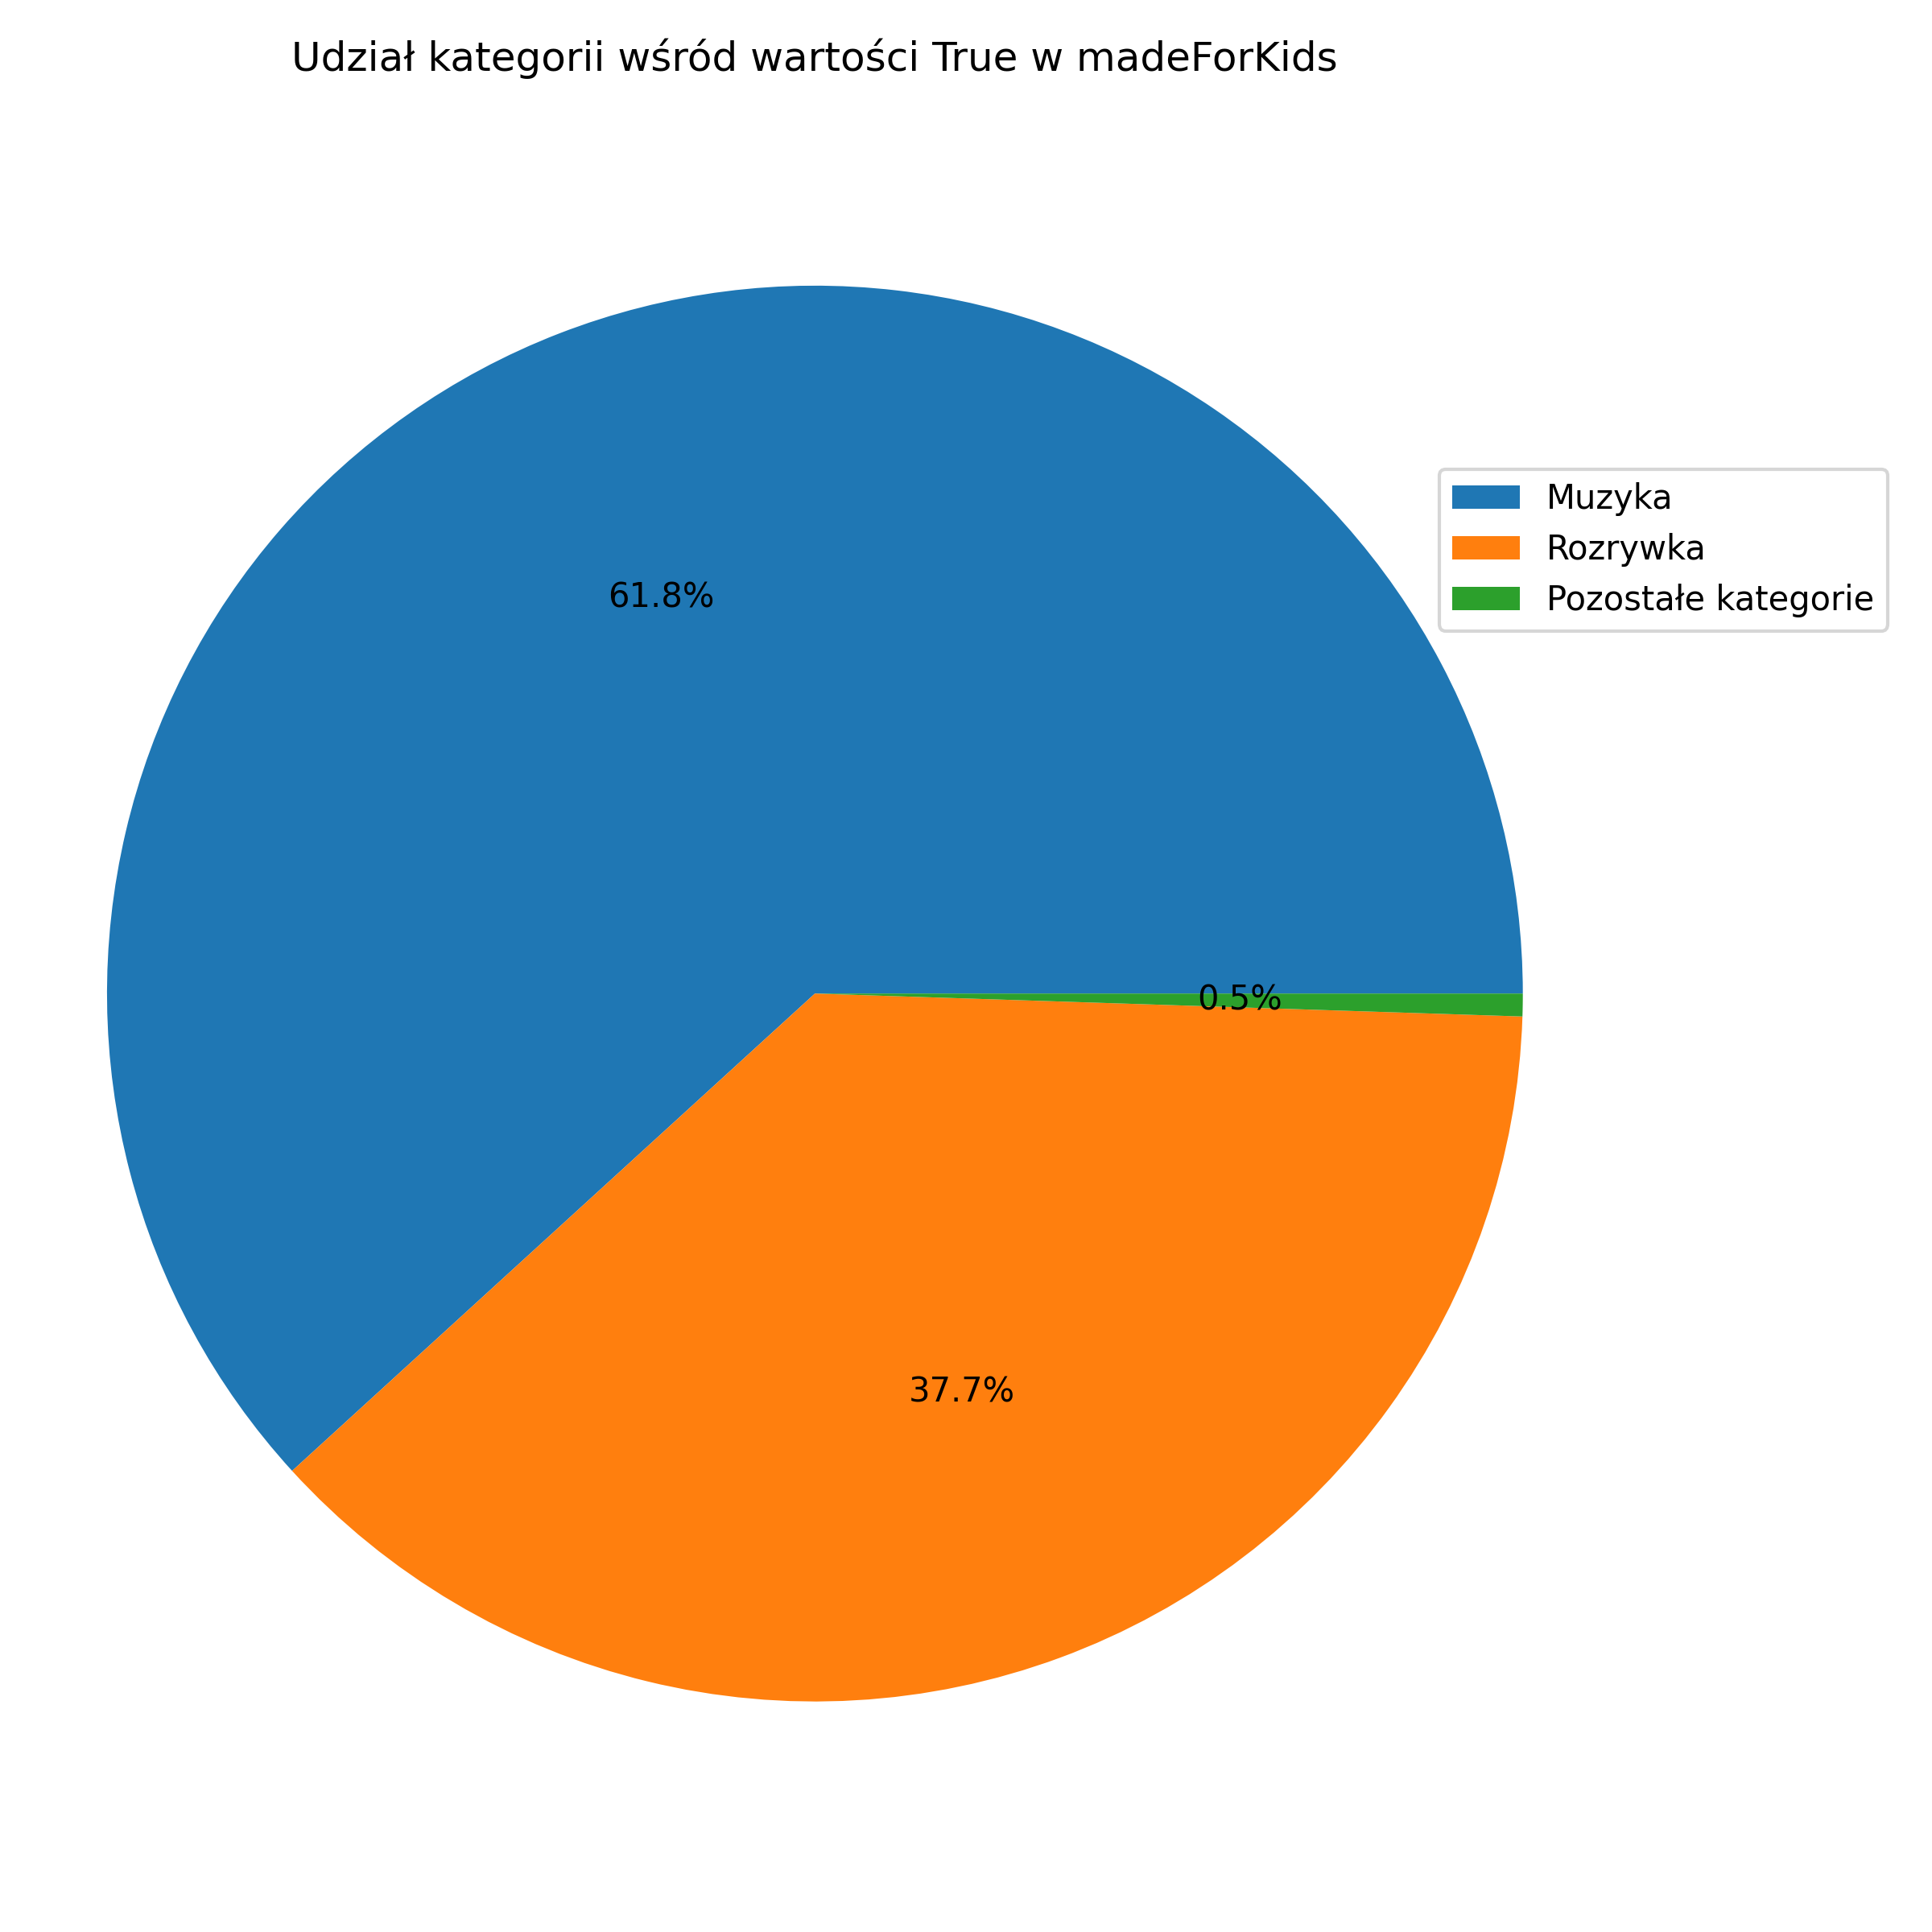
\includegraphics[width=0.5\textwidth]{Images/Diagram_true_do_reszty.png}
    \label{fig:madeforkids-true}
\end{figure}
Widzimy, że wartość true w atrybucie "Czy dla dzieci" pozwala nam w 99.5\% określić, że będą to dwie kategorie z pięciu, dokładniej mamy 61.8\% szans, że będzie to muzyka i 37.7\%, że będzie to rozrywka.

\begin{figure}[H]
    \centering
    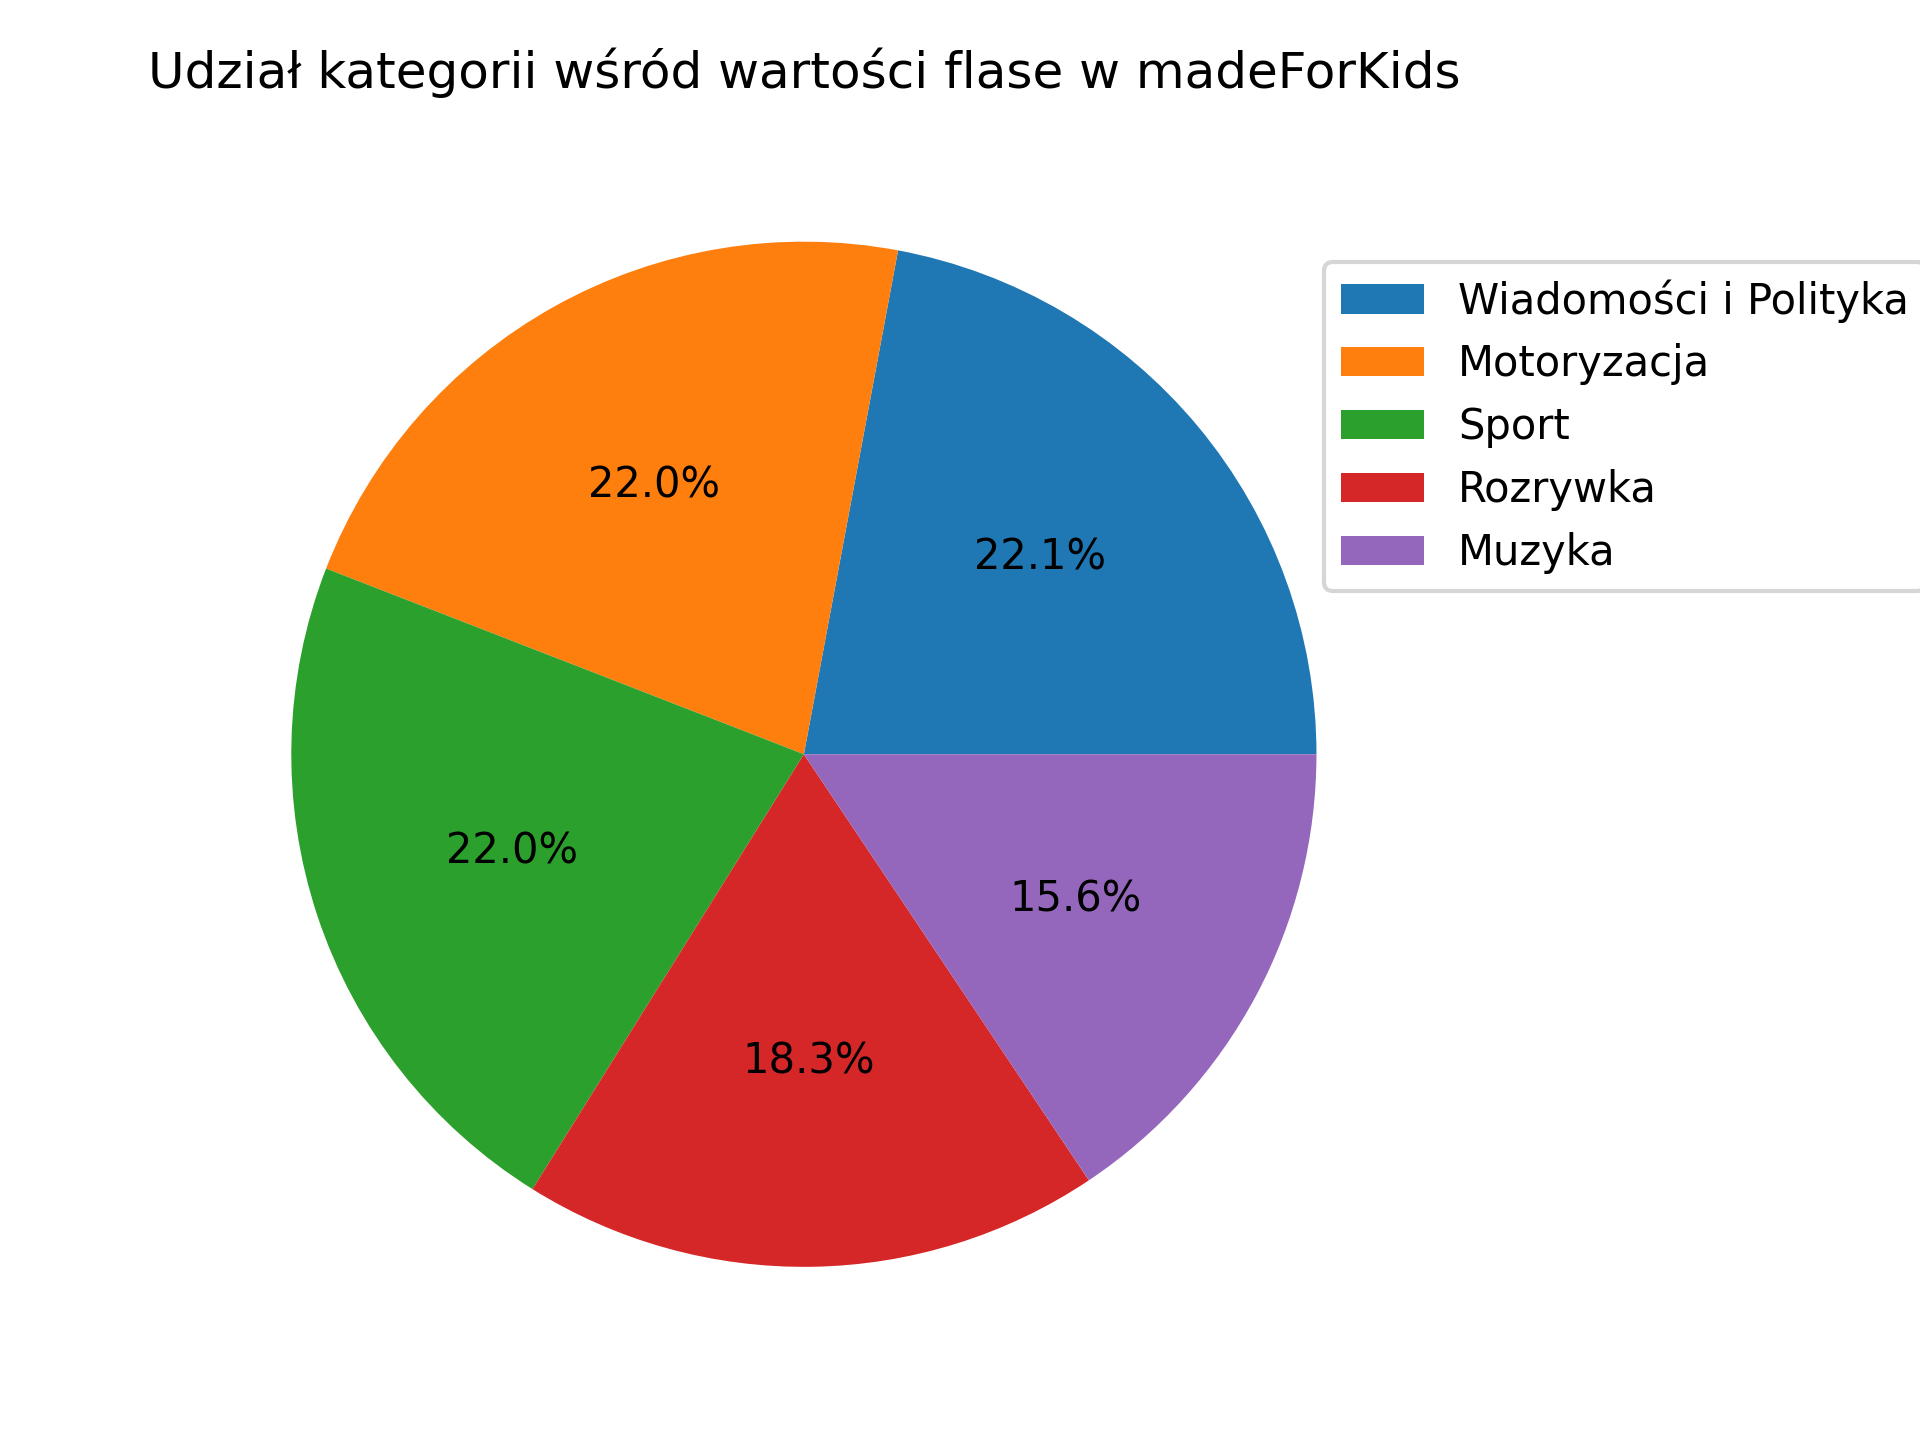
\includegraphics[width=0.5\textwidth]{Images/Diagram_false_do_reszty.png}
    \label{fig:madeforkids-false}
\end{figure}
Niestety dla wartości false widzimy, że nie ma tak znacznych różnic pomiędzy kategoriami.

\begin{figure}[H]
    \centering
    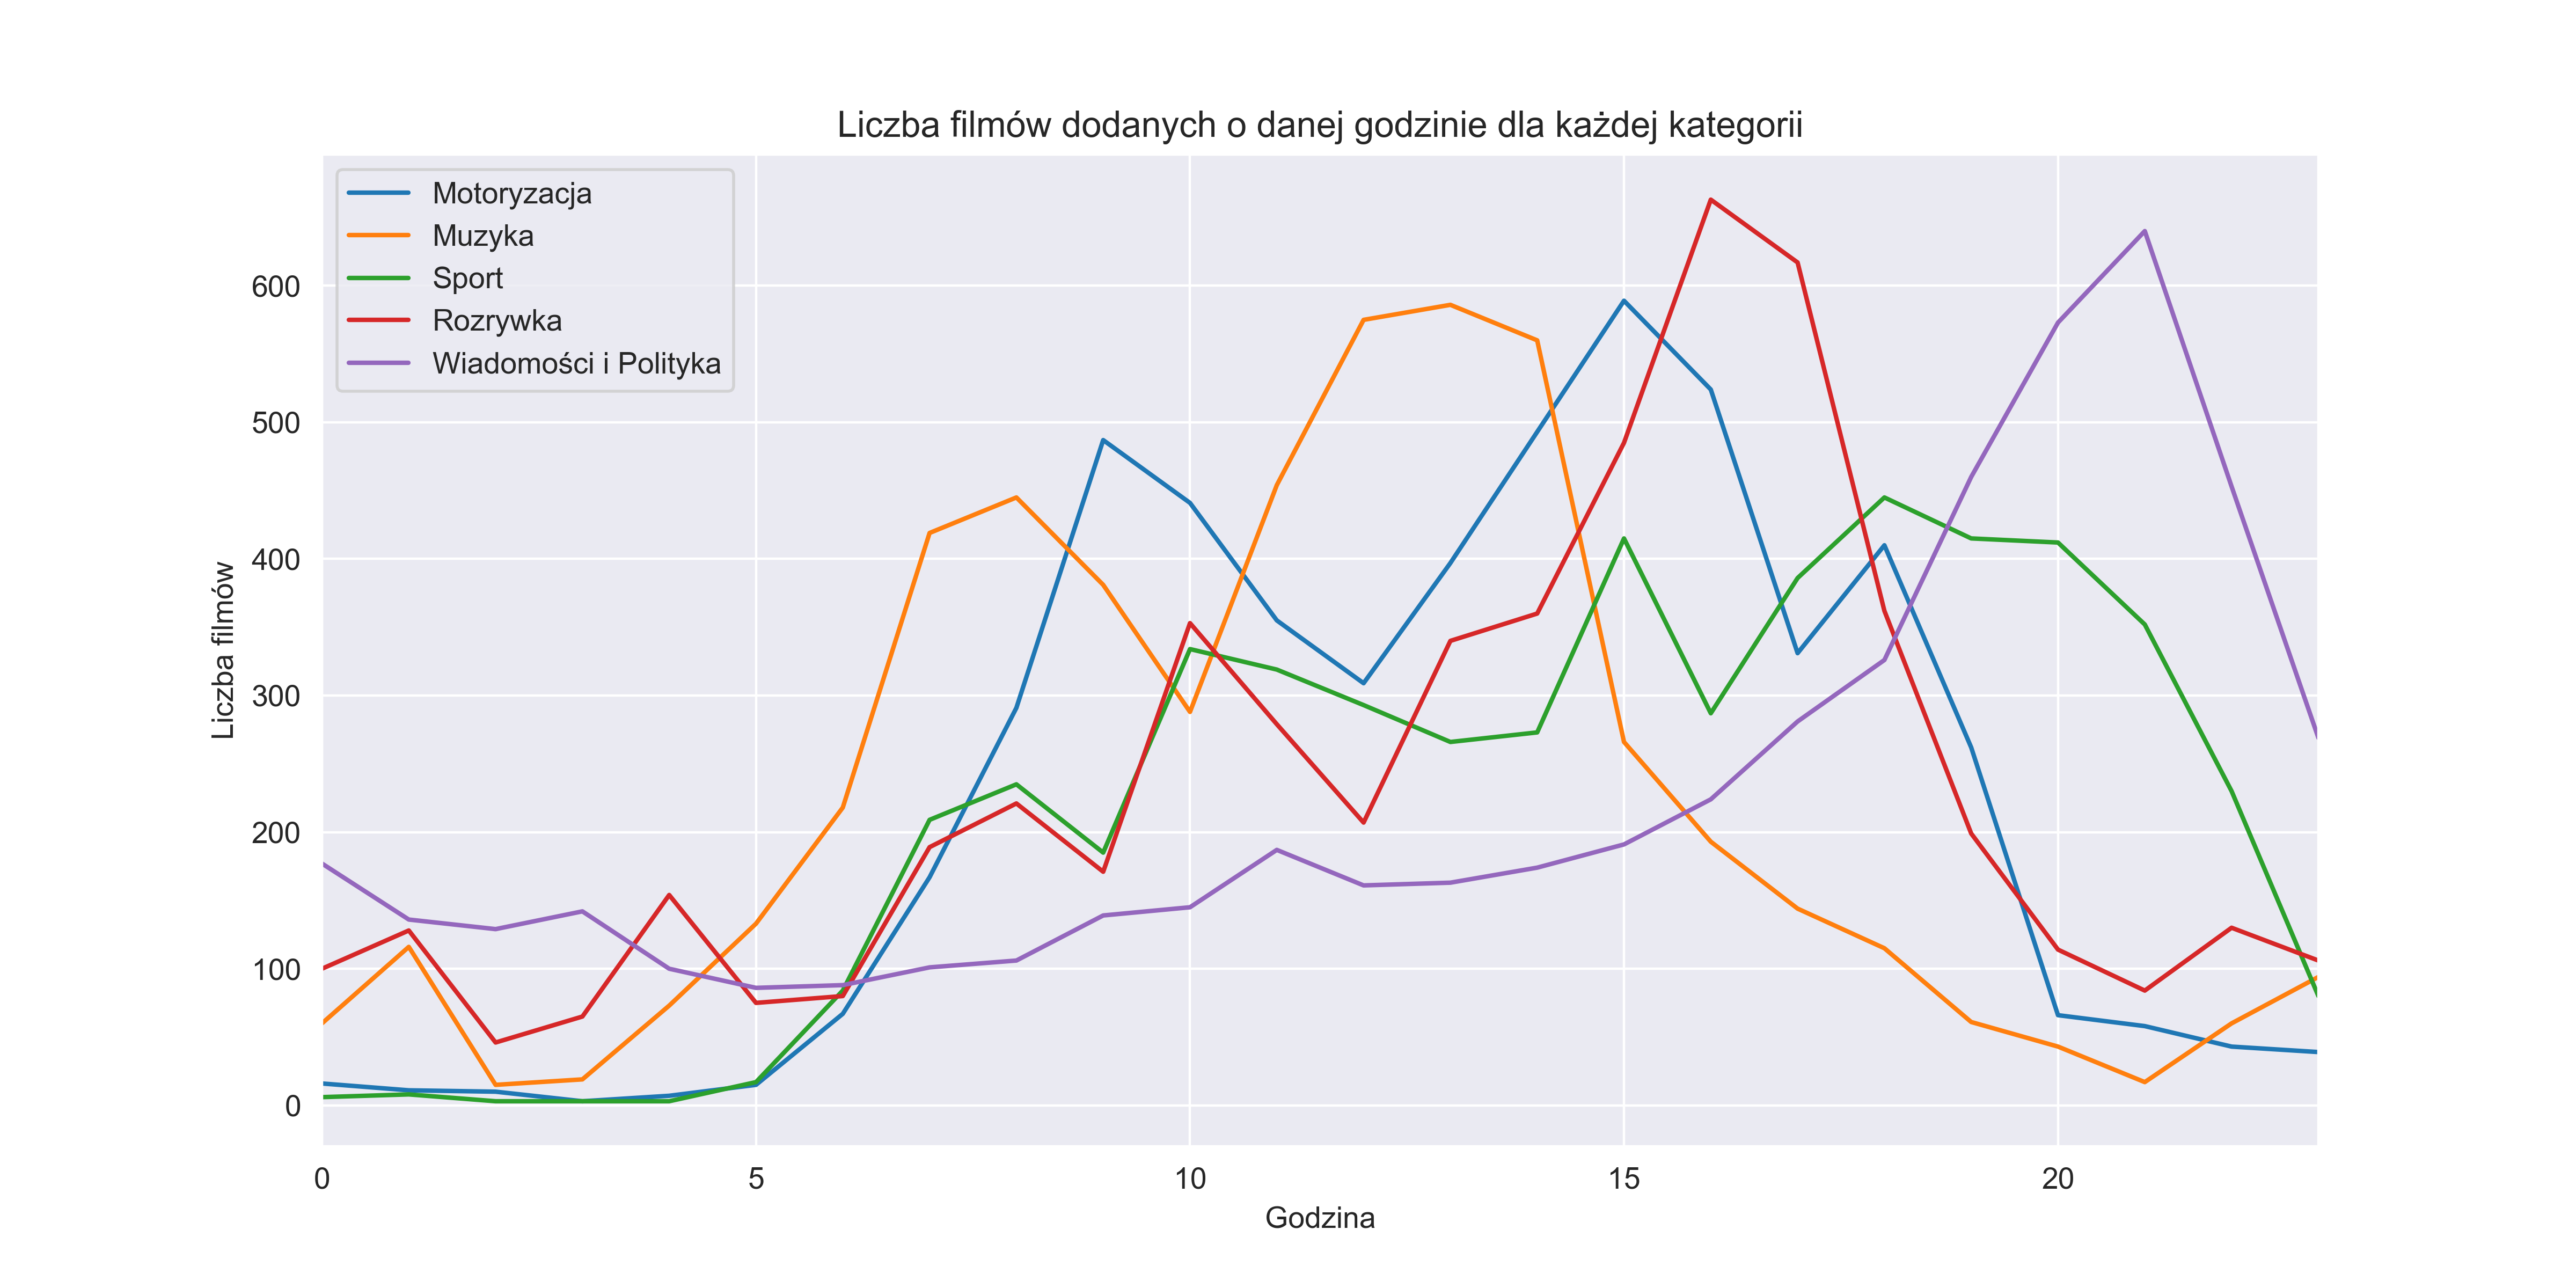
\includegraphics[width=0.5\textwidth]{Images/Zależność_dodania_do_filmu_a_kategorią.png}
    \label{fig:add_film_hour}
\end{figure}
Ten diagram bardzo dużo nam mówi o kategoriach, możemy się z niego dowiedzieć, że filmy z kategorii "Wiadomości i polityka" wrzucane są zazwyczaj w okolicach godziny 21. Natomiast kategoria sport nie ma jednej godziny, w której najczęściej wrzucane są filmy. Pozostałe trzy kategorie mają bardzo podobne wykresy z delikatnym przesunięciem.

\begin{figure}[H]
    \centering
    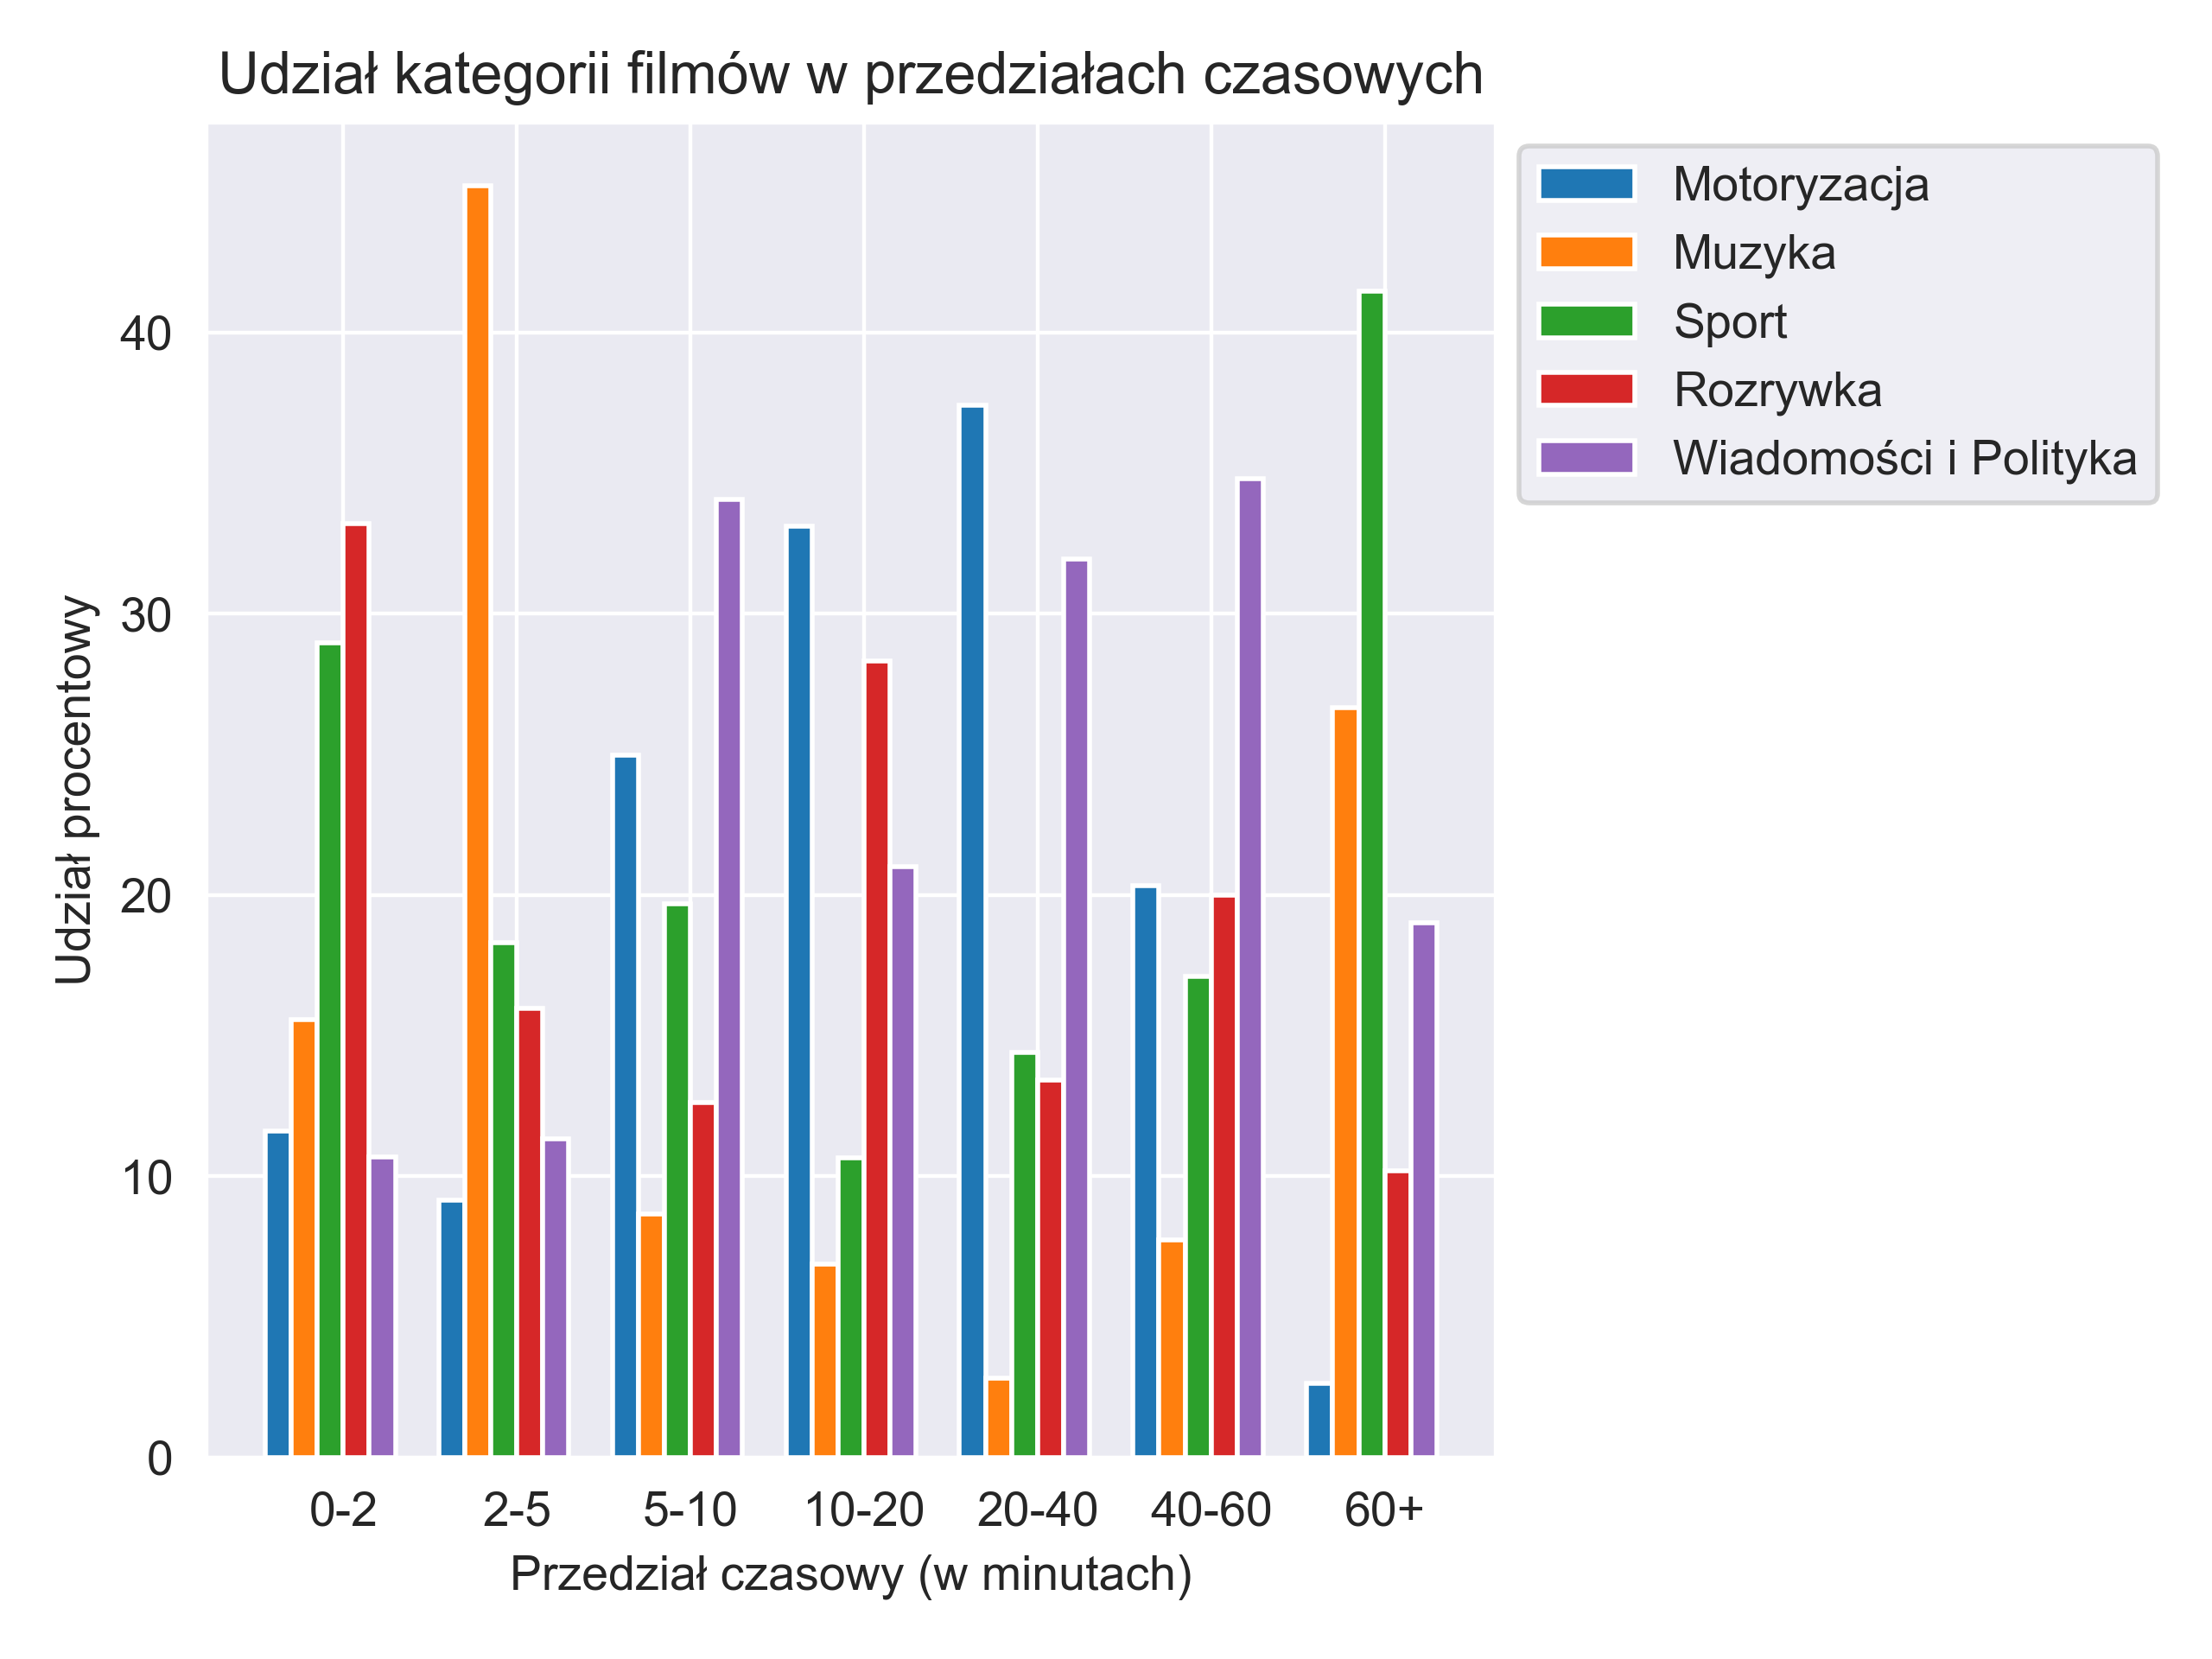
\includegraphics[width=0.5\textwidth]{Images/Udział kategorii filmów w przedziałach czasowych.png}
    \label{fig:durations}
\end{figure}
Wykres przedstawia udział poszczególnych kategorii w konkretnych przedziałach czasowych, co pozwala nam na przykład określić, że jeśli film trwa pomiędzy 2-5 minut, to na 45\% będzie to film z kategorii muzyka.


\begin{figure}[H]
    \centering
    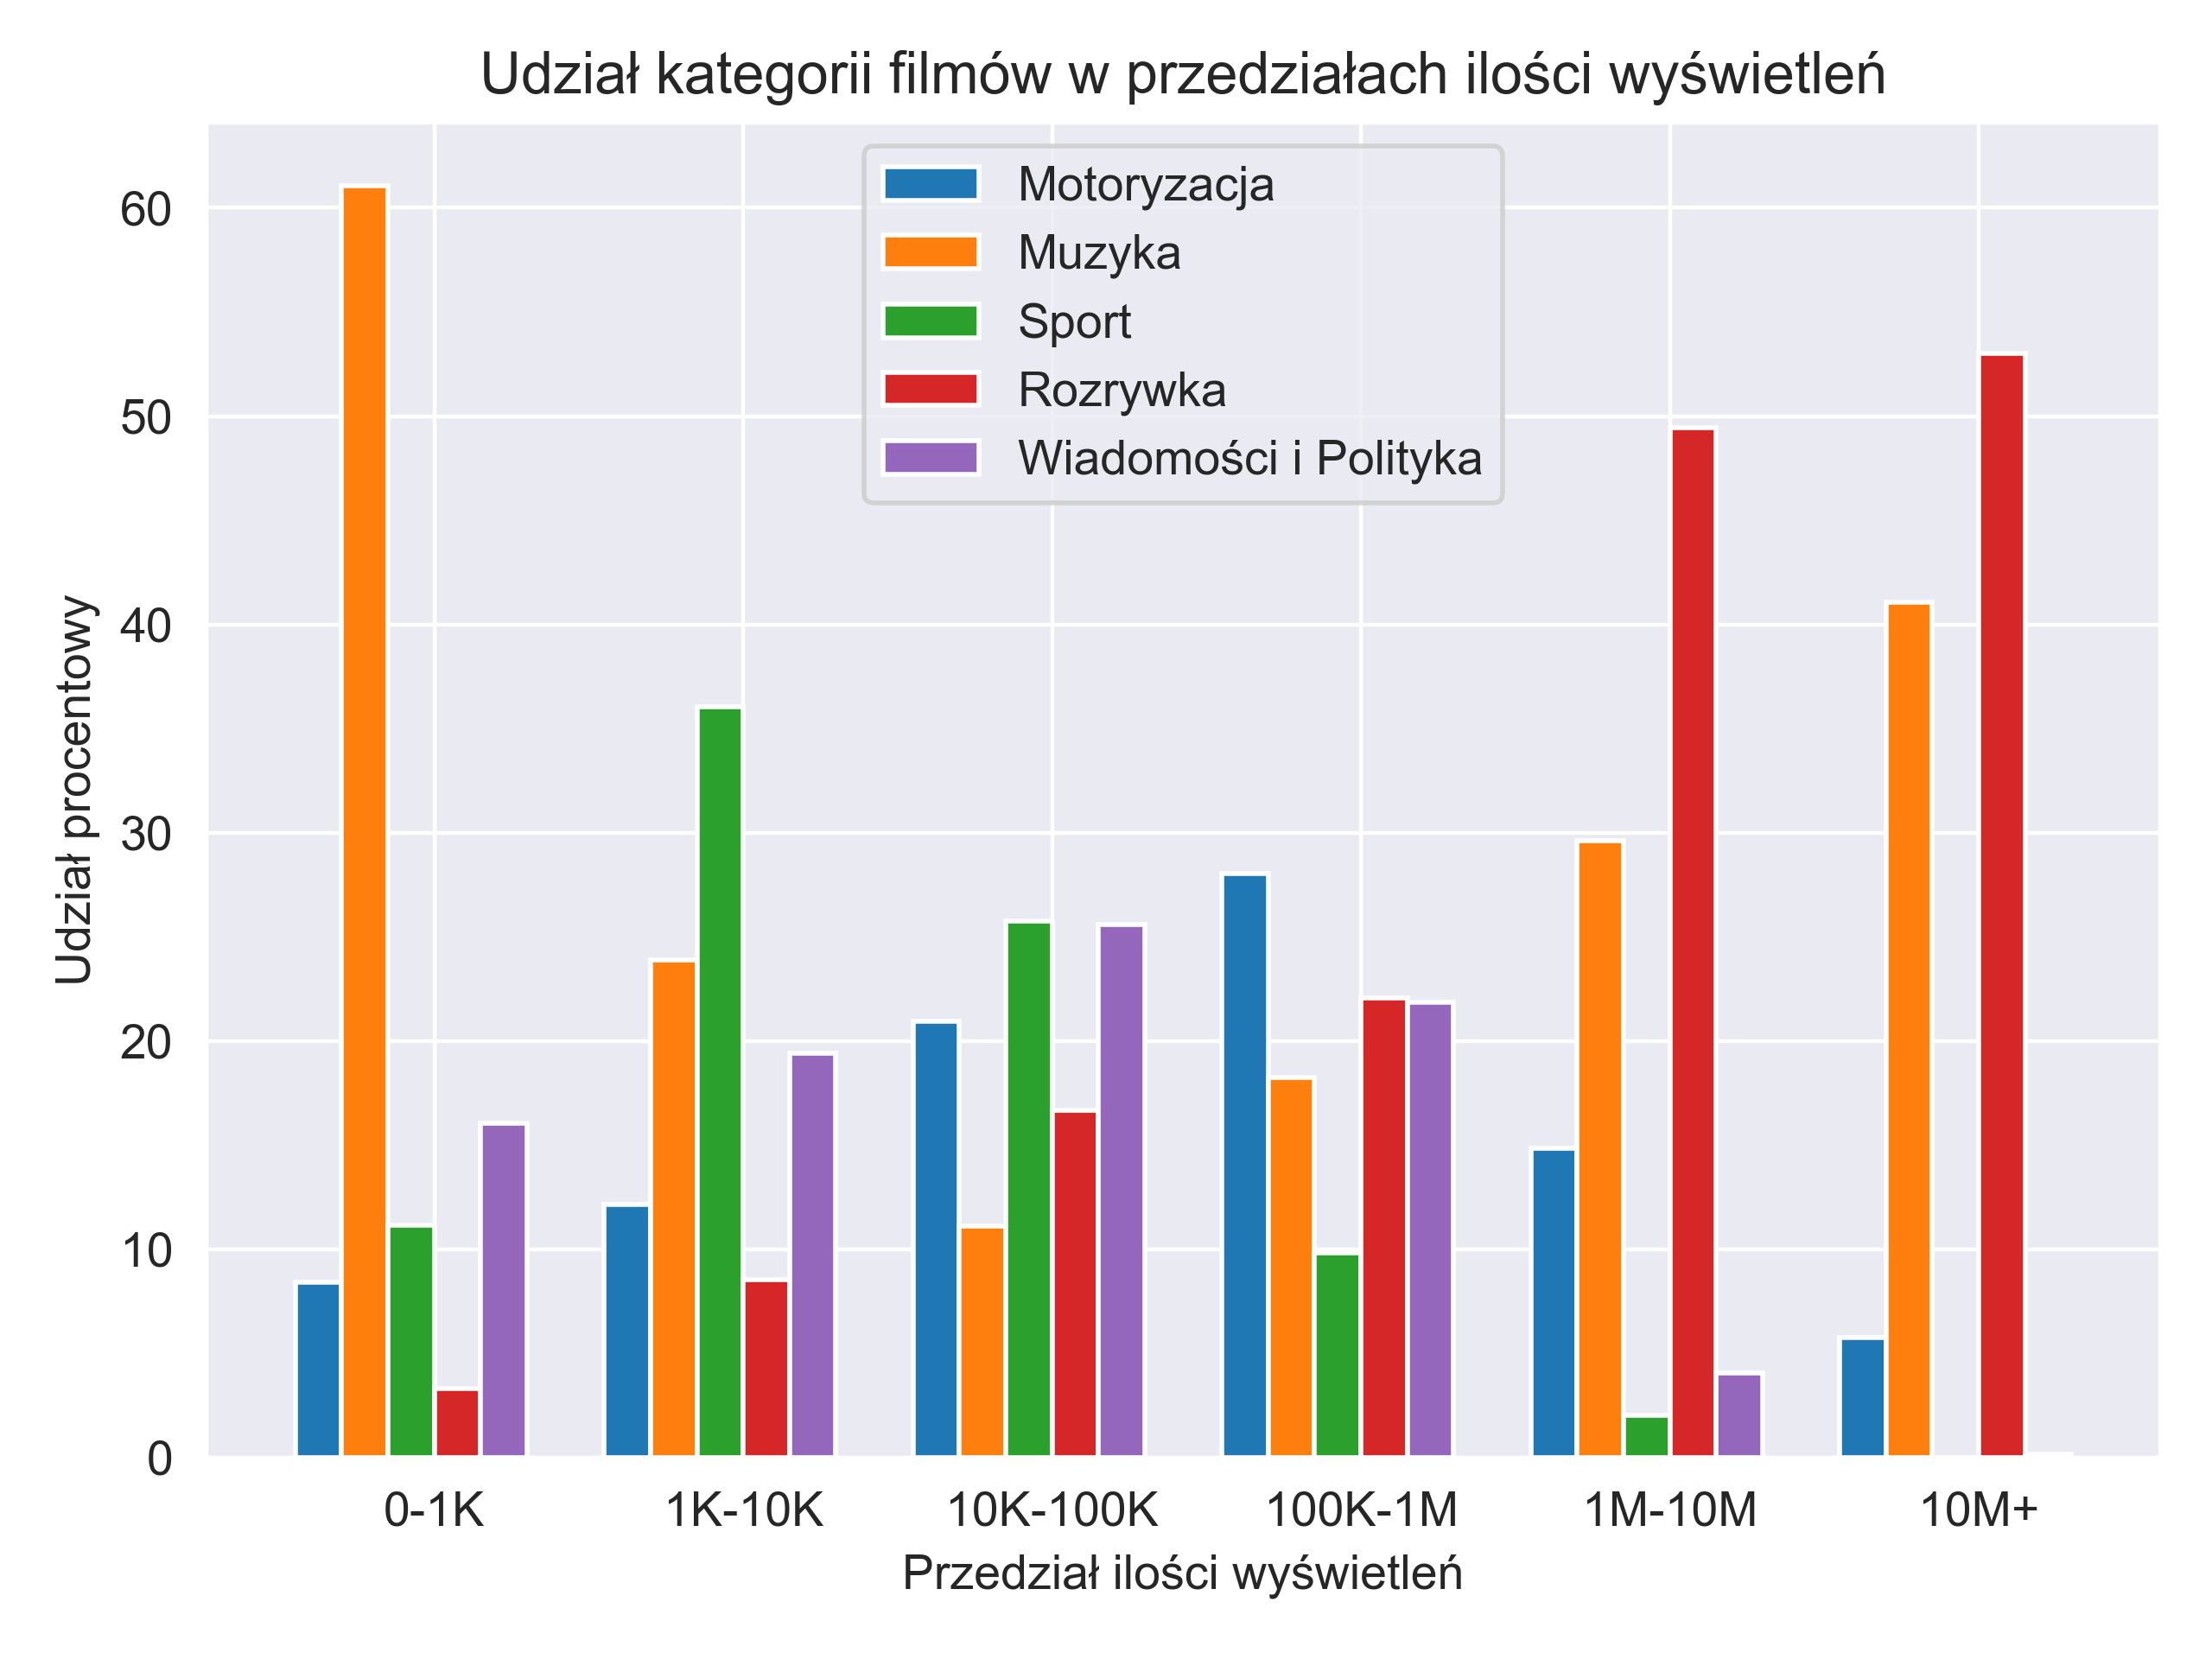
\includegraphics[width=0.5\textwidth]{Images/Zależność wyświetleń od kategorią.png}
    \label{fig:views_count}
\end{figure}
Następny diagram przedstawia zależność między kategoriami, a ilością wyświetleń w przedziałach. Widzimy, że środkowe przedziały dużo nam nie mówią, bo wszystkie kategorie mają podobną ilość wyświetleń, natomiast skrajne, takie jak 0-1k pozwalają nam dostrzec, że za 60\% wyświetleń w tym przedziale odpowiada kategoria muzyka lub, że w przedziale 10M+ nie występują kategorie Wiadomości i polityka oraz sport, a motoryzacja odpowiada tylko za 5\%.

\begin{figure}[H]
    \centering
    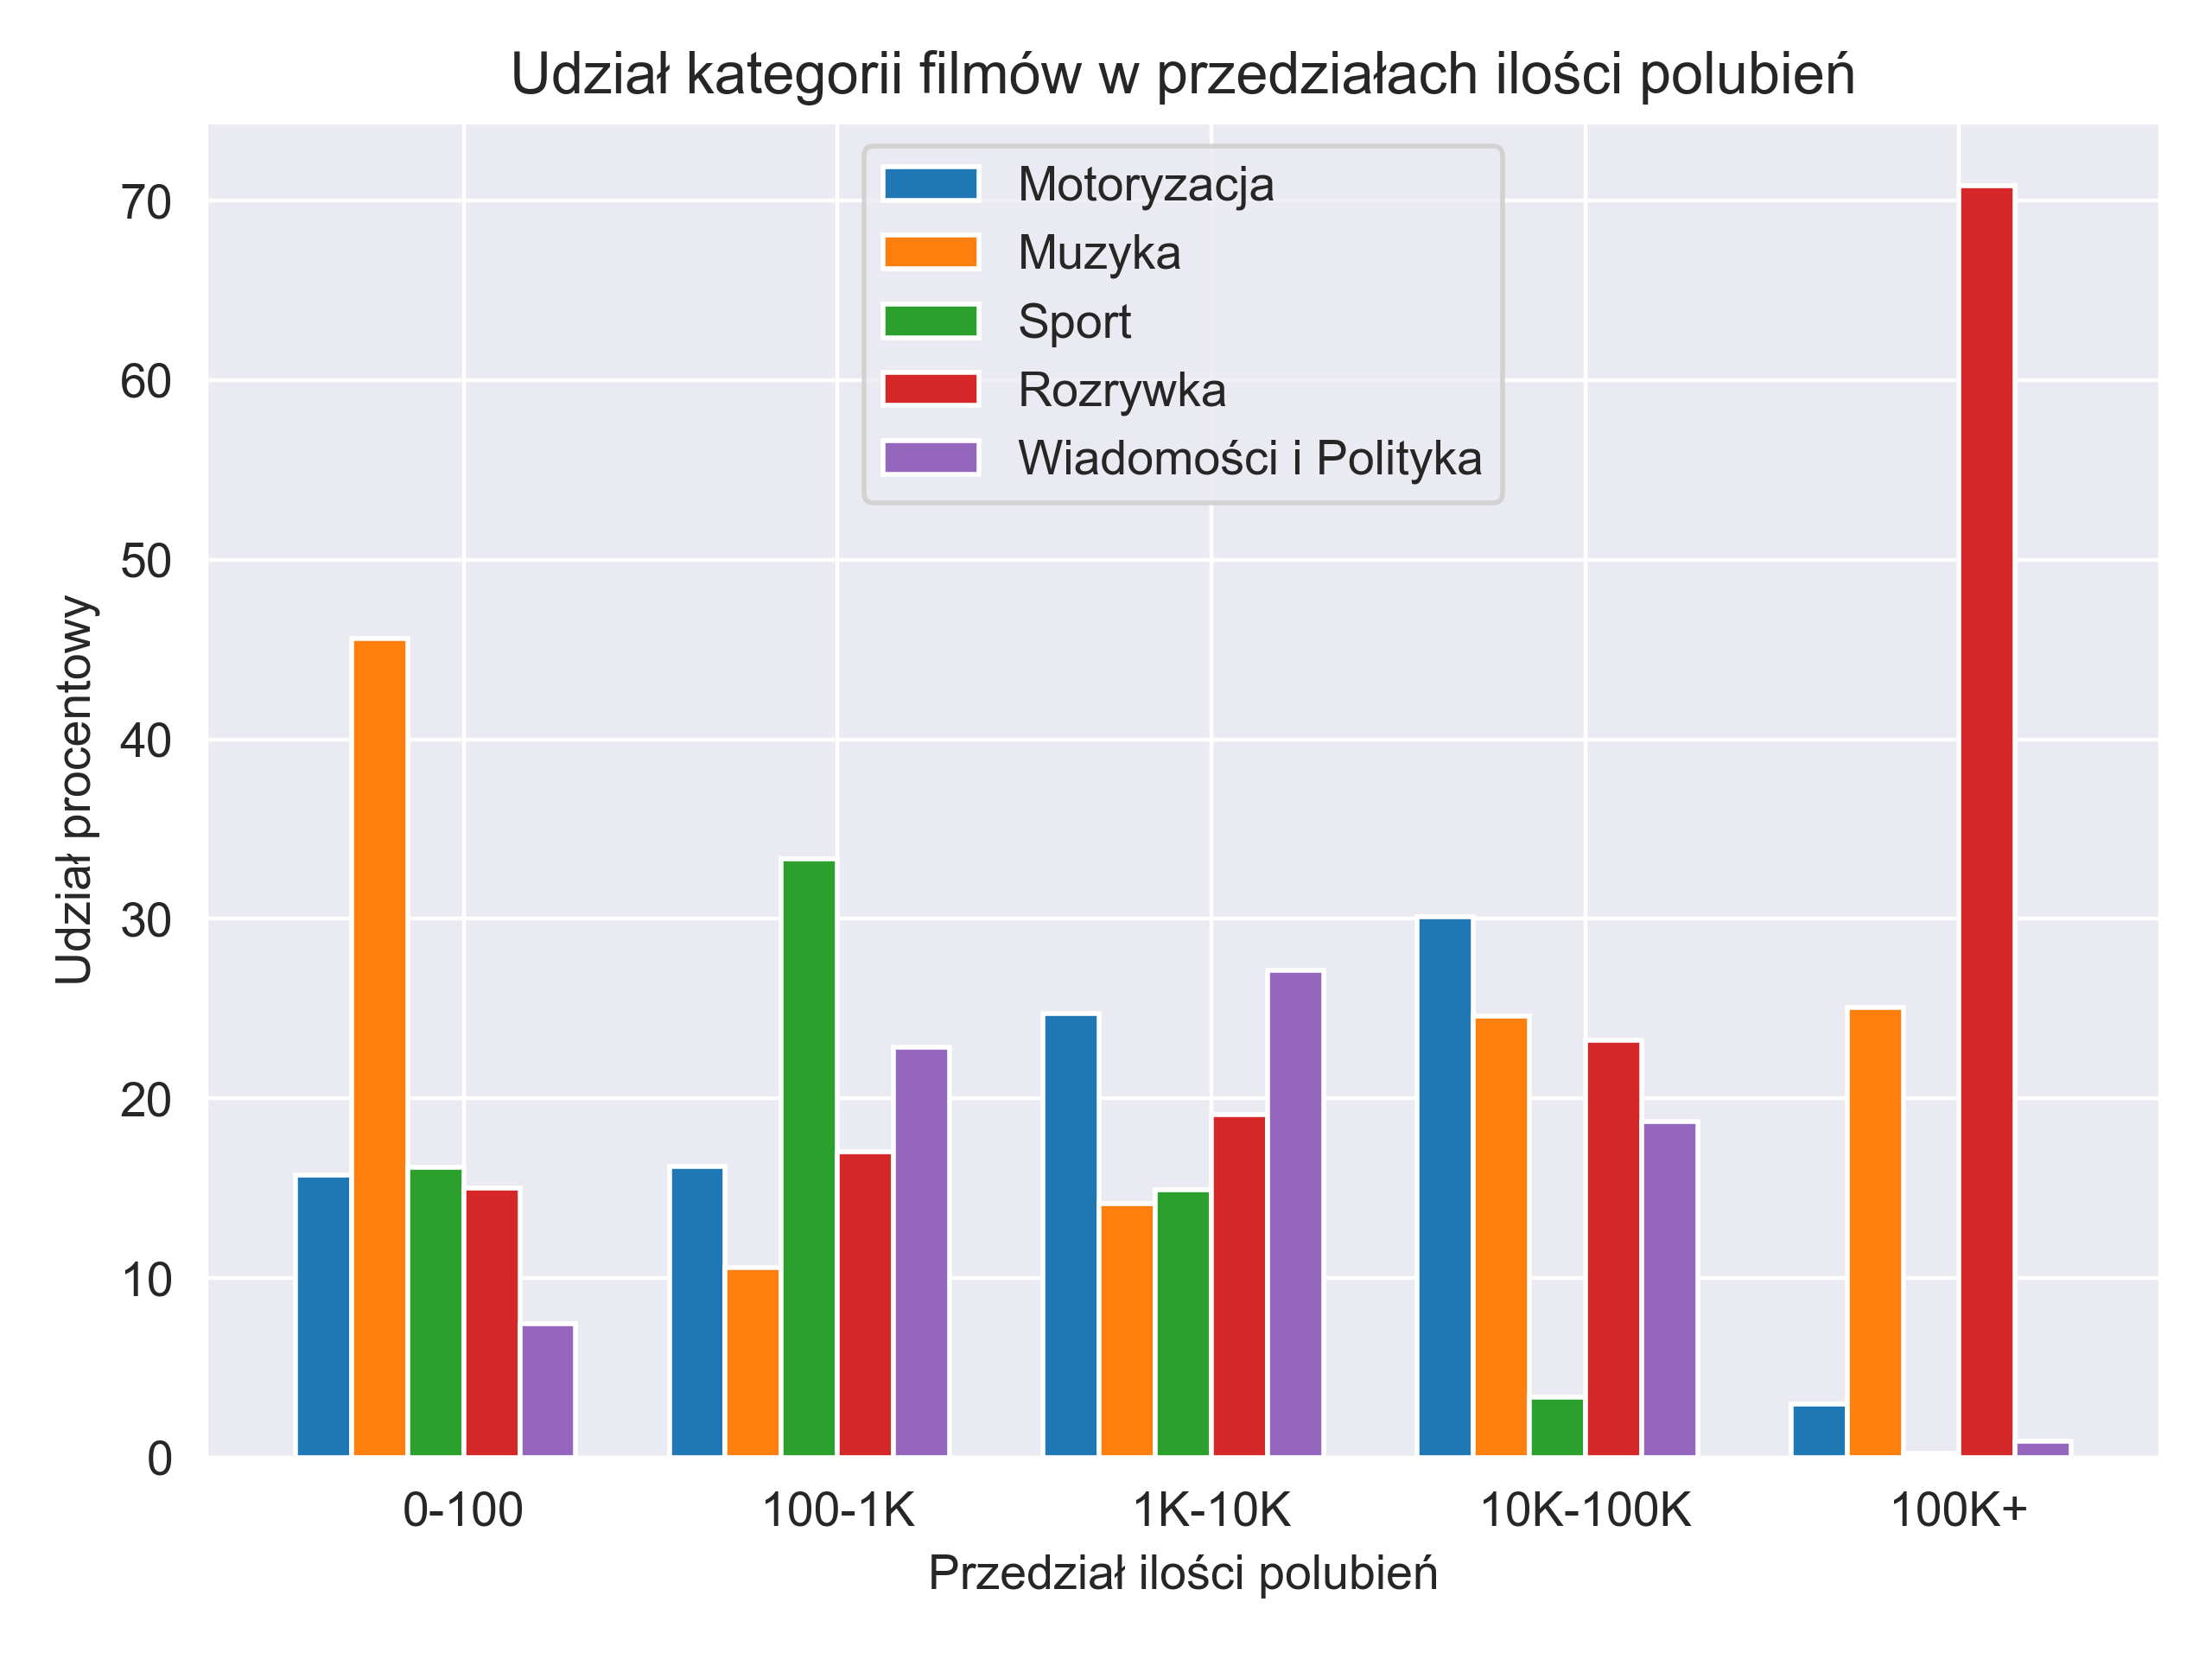
\includegraphics[width=0.5\textwidth]{Images/Zależność polubień od kategorią.png}
    \label{fig:likes_count}
\end{figure}
Ten diagram jest bardzo podobny do poprzedniego, ponieważ tutaj również nie widzimy dużych różnic pomiędzy kategoriami w środkowych przedziałach. Natomiast skrajne kategorie również dostarczają nam bardzo zróżnicowanych wyników, takich jak 70\% udziału kategorii rozrywka dla ilości polubień powyżej 100000.

\begin{figure}[H]
    \centering
    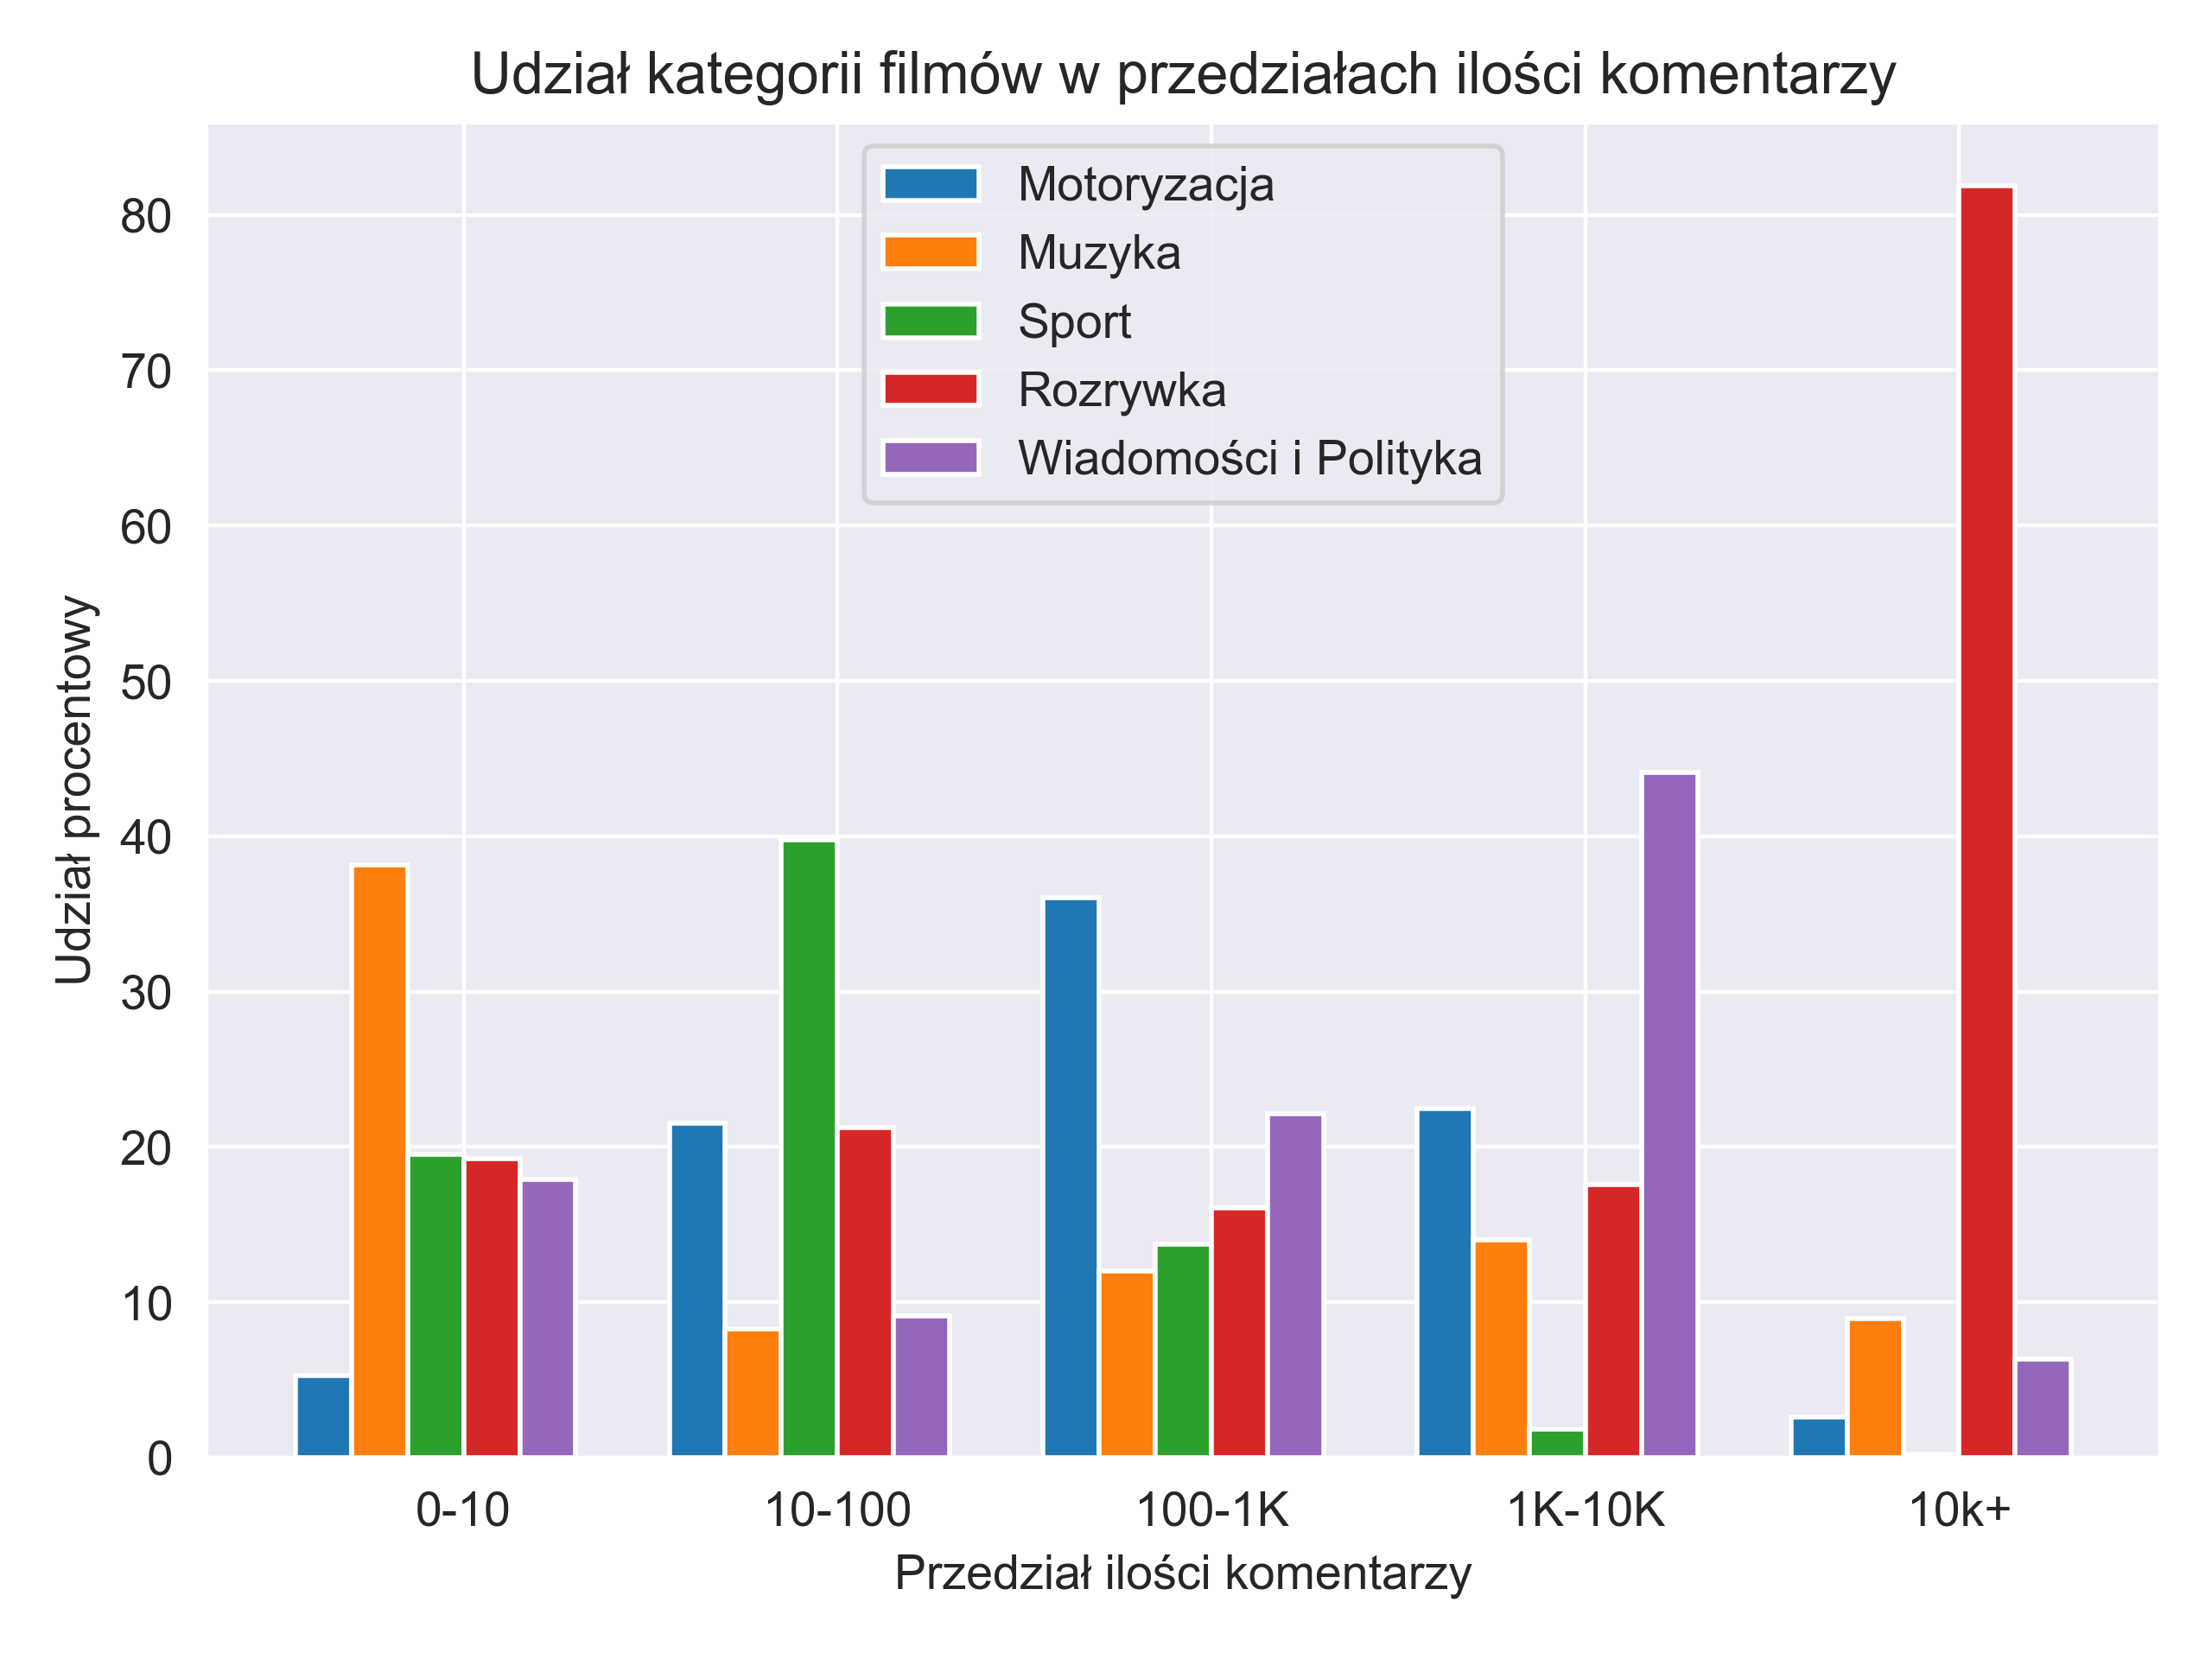
\includegraphics[width=0.5\textwidth]{Images/Zależność komentarzy od kategorią.png}
    \label{fig:coments_count}
\end{figure}
Przedostatni diagram przedstawiający zależność między atrybutami a kategoriami jest bardzo ciekawy, ponieważ tutaj w każdym przedziale inna kategoria dominuje o ponad 15\%. Jednak tak jak w dwóch ostatnich diagramach widać największą różnicę między kategoriami w górnym skrajnym przedziale, tak w tym przypadku jest to przedział ponad 10000, w którym kategoria rozrywka ma aż 80\% udziału.

\begin{figure}[H]
    \centering
    \includegraphics[width=0.5\textwidth]{Images/kategorię a dnia od 2012.png}
    \label{fig:add_days}
\end{figure}
Ostatni diagram przedstawia nam zależność między opublikowaniem filmu a kategorią. Możemy tutaj dostrzec, że zgromadzony przez nas zbiór nie jest idealny. Kategorie powinny się pokrywać, ponieważ codziennie są publikowane filmy z tych kategorii. Dlatego do uczenia naszego modelu nie bedziemy stosować tego atrybutu, tak aby nasz model był możliwy do wykorzystania dla najnowszych filmów i jak najlepiej działał na innych zbiorach.



\section{Przygotowanie modelu}
% Delete the text and write your Results here:
%------------------------------------

\subsection{DecisionTreeClassifier}
\label{DTC}
\hspace{\parindent}
DecisionTreeClassifier jest algorytmem uczenia maszynowego, który opiera się na drzewach decyzyjnych do problemów klasyfikacji. Jest to jeden z najprostszych i najbardziej intuicyjnych algorytmów uczenia maszynowego.

Drzewo decyzyjne składa się z węzłów i krawędzi, które reprezentują decyzje oparte na wartościach cech. Algorytm uczący DecisionTreeClassifier tworzy drzewo decyzyjne na podstawie dostępnych danych treningowych, które składają się z przykładów oznaczonych etykietami klas.

Algorytm działa następująco:
\begin{enumerate}
    \item Wybór najlepszej cechy, która podzieli zbiór danych na sposób, który najlepiej separuje przykłady klas.
    \item Podział danych na podstawie wartości wybranej cechy, tworzący węzeł decyzyjny.
    \item Powtarzanie kroków 1-2 rekurencyjnie dla każdego nowo utworzonego węzła, aż zostaną spełnione pewne kryteria stopu.
    \item Przypisanie etykiety klasy do liści drzewa na podstawie większościowych etykiet przykładów uczących w danym liściu.
\end{enumerate}

\subsection{RandomForestClassifier}
\label{RFC}
\hspace{\parindent}
RandomForestClassifier jest algorytmem uczenia maszynowego, który opiera się na zasadzie ensemble learning, czyli łączeniu wyników wielu modeli w celu uzyskania lepszej jakości predykcji. Jest oparty na metodzie drzew decyzyjnych.

RandomForestClassifier tworzy wiele drzew decyzyjnych na podstawie losowych podzbiorów danych treningowych. Każde drzewo jest trenowane niezależnie na różnych podzbiorach danych. Podczas prognozowania klasyfikacji każde drzewo decyzyjne w lesie przewiduje wynik, a ostateczna predykcja jest dokonywana na podstawie głosowania większości.

Ważną cechą RandomForestClassifier jest wprowadzenie losowości poprzez losowe wybieranie podzbiorów cech do trenowania każdego drzewa. Dzięki temu zapobiega się overfittingowi (przeuczeniu), gdy model zbytnio dopasowuje się do danych treningowych.

Dodatkowo, podczas trenowania każdego drzewa, stosuje się losowanie ze zwracaniem, co oznacza, że każdy podzbiór danych ma możliwość zawierać duplikaty próbek. Ta technika znana jako bagging (bootstrap aggregating) pomaga zwiększyć różnorodność drzew w lesie i zmniejszyć wariancję modelu.

\subsection{Przygotowanie modelu dla naszego zbioru}
\hspace{\parindent}

Nasze dane podzielimy na zbiór treningowy i testowy w stosunku 1:3, co pozwoli na odpowiednie nauczenie modelu.

Po wytrenowaniu naszego modelu oraz wytestowaniu go otrzymujemy następujące wyniki:
\begin{table}[htbp]
\centering
\caption{Wyniki F1-score dla różnych modeli}
\label{tab:results}
\begin{tabular}{|l|c|c|c|c|}
\hline
\multirow{2}{*}{Model} & \multicolumn{4}{c|}{F1-score} \\
\cline{2-5}
& Motoryzacja & Muzyka & Sport & Rozrywka \\
\hline
DTC & 0.67 & 0.75 & 0.69 & 0.68 \\
\hline
RFC & 0.76 & 0.84 & 0.79 & 0.79 \\
\hline
\end{tabular}

\vspace{10pt}

\begin{tabular}{|l|c|c|c|c|}
\hline
\multirow{2}{*}{Model} & \multicolumn{4}{c|}{F1-score} \\
\cline{2-5}
& WiP & Dokładność & Arytmetyczna & Ważona \\
\hline
DTC & 0.85 & 0.73 & 0.73 & 0.73 \\
\hline
RFC & 0.9 & 0.82 & 0.82 & 0.82 \\
\hline
\end{tabular}
\end{table}

WiP\footnote{Wiadmości i polityka}

F1-score jest miarą oceny jakości klasyfikacji. Jest to średnia harmoniczna precyzji (precision) i czułości (recall) klasyfikatora. Czułość to miara, która mierzy zdolność klasyfikatora do wykrywania rzeczywiście pozytywnych przypadków, podczas gdy precyzja ocenia, ile zidentyfikowanych jako pozytywne przypadków jest faktycznie poprawnych.

Dokładność (accuracy) to miara, która mierzy ogólną skuteczność klasyfikatora poprzez porównanie liczby poprawnie sklasyfikowanych przypadków do całkowitej liczby przypadków. Średnia arytmetyczna (macro avg) to miara dla każdej klasy, niezależnie od rozmiaru klasy. Średnia ważona (weighted avg) to miara dla każdej klasy, z wagami proporcjonalnymi do liczności klas. Ponieważ w zbiorze mamy bardzo zbliżoną liczbę rekordów poszczególnych kategorii, dlatego wyniki w tych polach są w przybliżeniu taki same.

Jak widzimy na tabelce nasze modele najlepiej radzą sobie w przewidywaniu wiadomości i polityki oraz nieco gorzej radzą sobie z muzyką.

Ogólnie również możemy zaobserwować, że model RFC radzi sobie lepiej aż o 9 punktów procentowych niż model DTC, który uzyskuje wynik na poziomie 73\%.

Nasze dane możemy również zaprezentować za pomocą macierzy pomyłek: 

\begin{figure}[H]
    \centering
    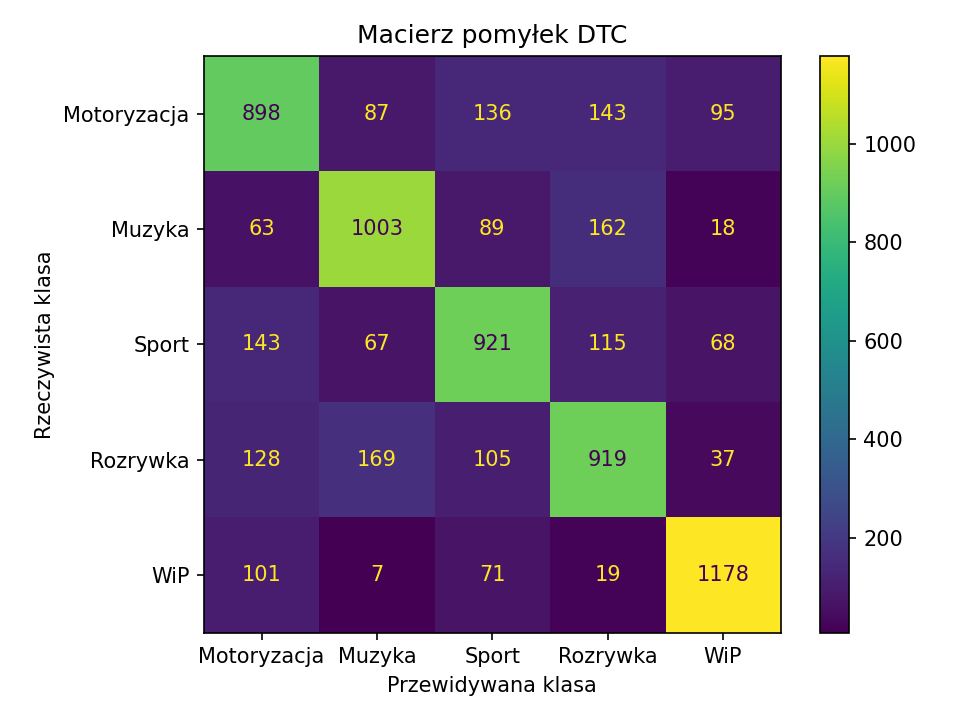
\includegraphics[width=0.5\textwidth]{Images/klasyfikacja DTC.png}
    \label{fig:DTC}
\end{figure}

\begin{figure}[H]
    \centering
    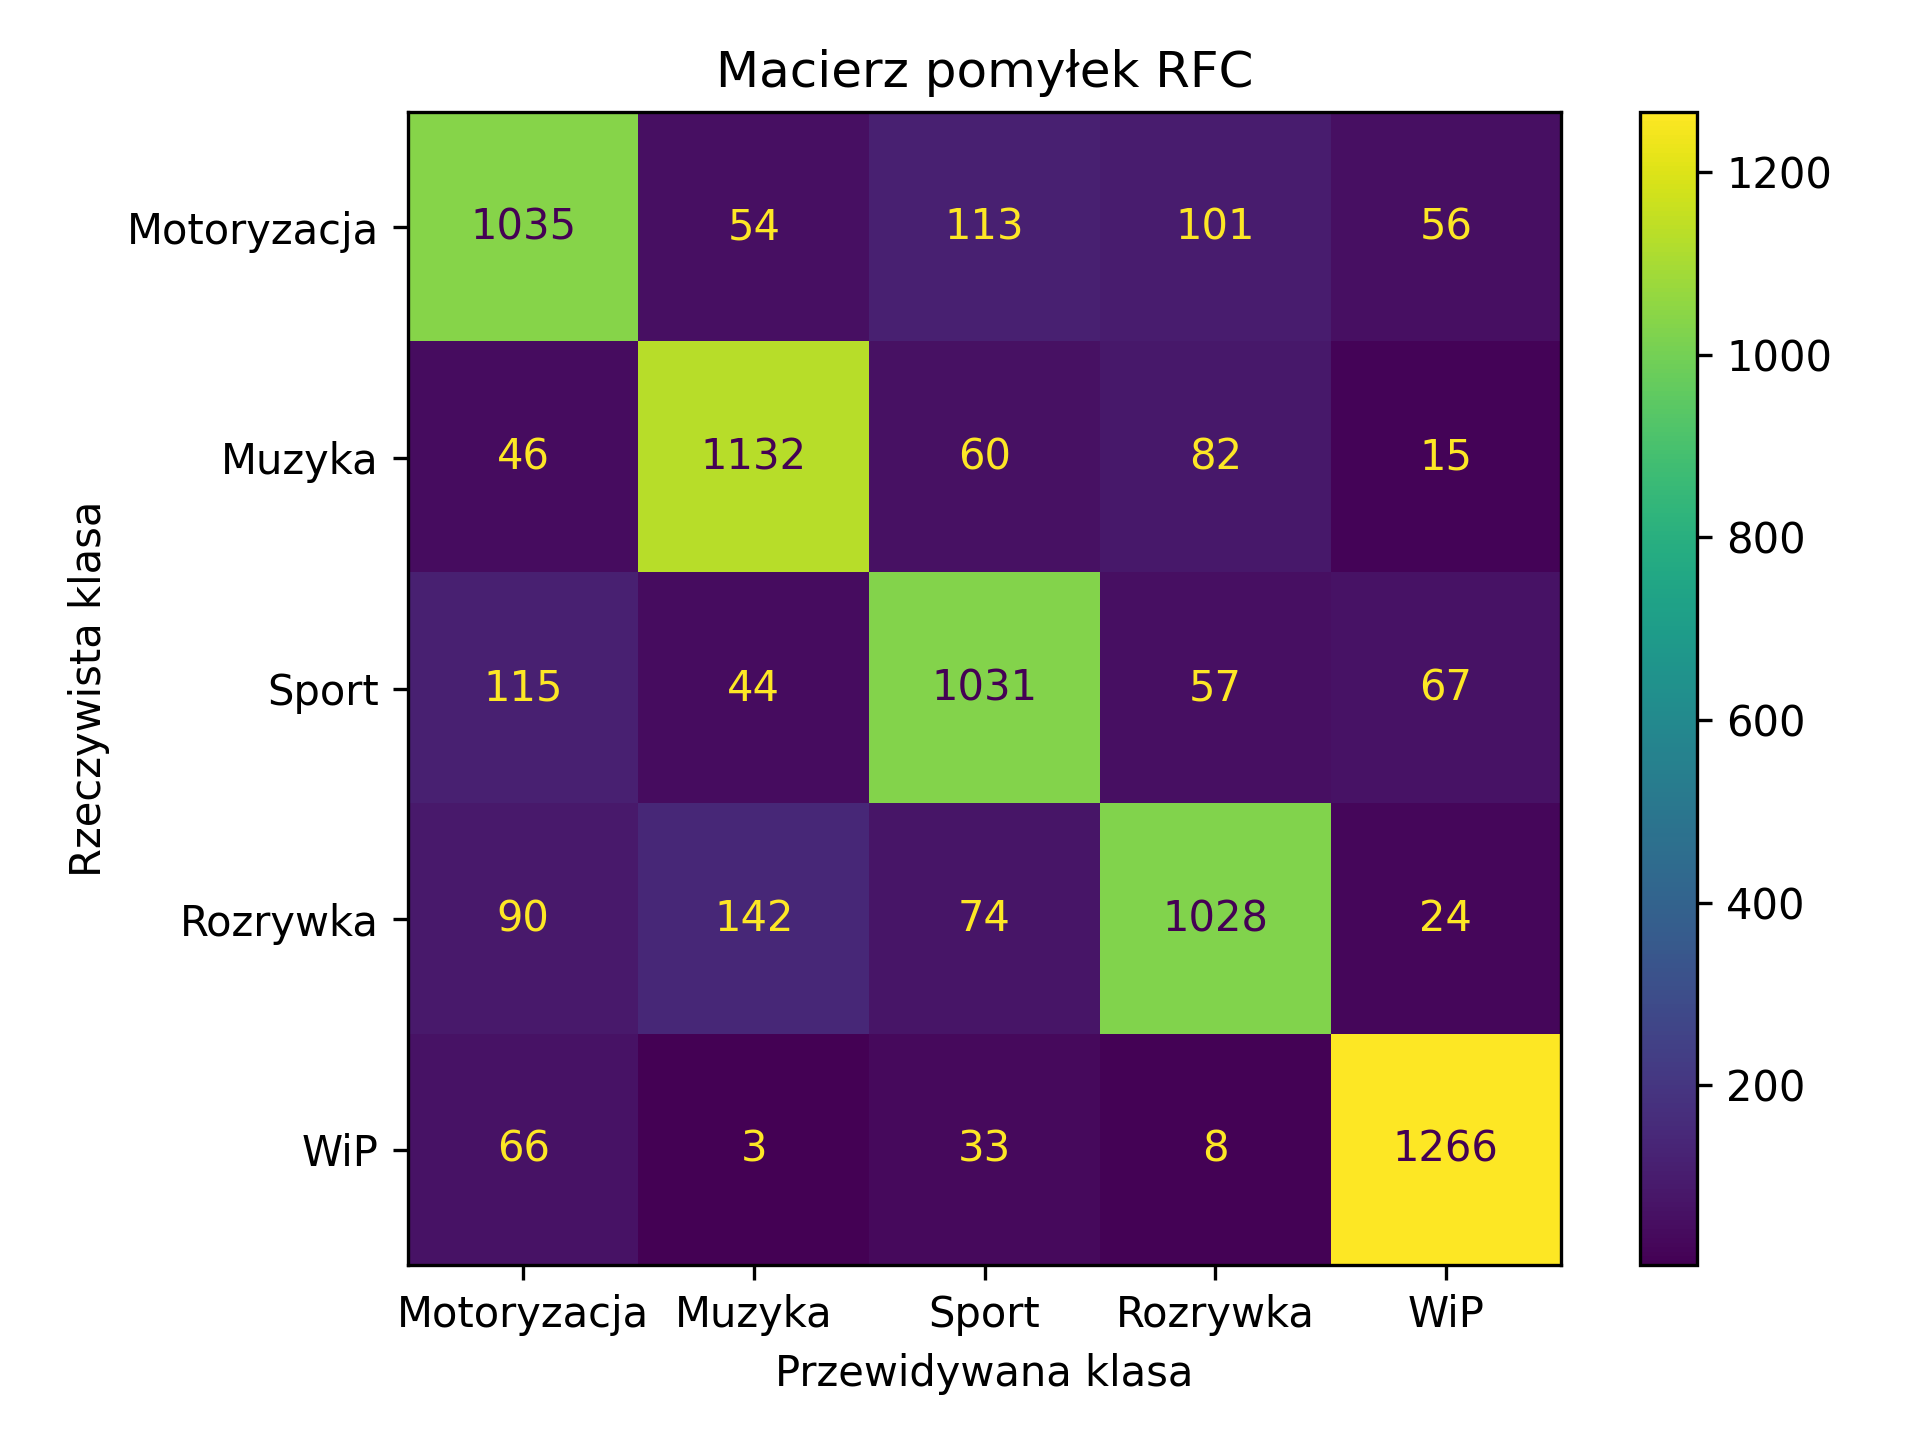
\includegraphics[width=0.5\textwidth]{Images/klasyfikacja RFC.png}
    \label{fig:RFC}
\end{figure}

Na macierzy pomyłek możemy zobaczyć dokładnie, ile razy model przewidywał jakąś kategorię, a jaka była naprawdę.

Warto sprawdzić czy, nasz model nie poradzi sobie lepiej bez jakiegoś atrybutu przy klasyfikacji:


\begin{table}[htbp]
\centering
\label{tab:results}
\rotatebox{90}{
\begin{tabular}{|l|c|c|c|c|c|c|c|}
\hline
\multirow{2}{*}{Model} & \multirow{2}{*}{Bez} & \multicolumn{6}{c|}{F1-score} \\
\cline{3-8}
& &Motoryzacja & Muzyka & Sport & Rozrywka & Wip & Dokładność \\
\hline
\multirow{6}{*}{DTC} &  Liczba Wyświetleń & 0.62 & 0.73 & 0.63 & 0.66 & 0.78 & 0.69 \\
\cline{2-8}
& Liczba komentarzy & 0.58 & 0.74 & 0.61 & 0.65 & 0.62 & 0.64 \\
\cline{2-8}
& Liczba polubień & 0.59 & 0.72 & 0.63 & 0.67 & 0.83 & 0.69\\
\cline{2-8}
& Czy dla dzieci & 0.67 & 0.73 & 0.69 & 0.67 & 0.83 & 0.72 \\
\cline{2-8}
& Czas trwania & 0.57 & 0.69 & 0.63 & 0.59 & 0.81 & 0.66 \\
\cline{2-8}
& Minuty po północy & 0.61 & 0.71 & 0.66 & 0.62 & 0.82 & 0.68 \\
\hline
\multirow{6}{*}{RFC} &  Liczba Wyświetleń & 0.73 & 0.81 & 0.72 & 0.75 & 0.85 & 0.77 \\
\cline{2-8}
& Liczba komentarzy & 0.69 & 0.8 & 0.71 & 0.75 & 0.71 & 0.73\\
\cline{2-8}
& Liczba polubień & 0.68 & 0.79 & 0.7 & 0.76 & 0.89 & 0.77 \\
\cline{2-8}
& Czy dla dzieci & 0.76 & 0.82 & 0.78 & 0.77 & 0.89 & 0.8\\
\cline{2-8}
& Czas trwania & 0.68 & 0.75 & 0.73 & 0.66 & 0.87 & 0.74 \\
\cline{2-8}
& Minuty po północy & 0.69 & 0.79 & 0.73 & 0.71 & 0.88 & 0.76\\
\hline
\end{tabular}}
\vspace{15pt}
\end{table}

\newpage
Z tabelki możemy odczytać, że każdy z argumentów polepsza naszą klasyfikację, nawet "czy dla dzieci", chociaż są to tylko 2 punkty procentowe, ale bardzo dla nas ważne.






\section{Wnioski}
% Delete the text and write your Discussion here:
%------------------------------------

Przedstawione eksperymenty wskazały, że nasze modele bardzo dobrze sobie radzą z klasyfikacją kategorii od parametrów filmów. Raport wskazuje również na zależność między wszystkimi atrybutami a kategorią. 

Warto również zauważyć, że nasze badania uwzględniały różne metody klasyfikacji, takie jak Random Forest Classifier \ref{RFC} oraz Decision Tree Classifier \ref{DTC}. Porównując wyniki obu modeli, stwierdziliśmy, że model RFC radzi sobie znacznie lepiej niż model DTC. Różnica w wynikach między nimi wynosi aż 9 punktów procentowych, co sugeruje, że model RFC jest bardziej efektywny w klasyfikacji kategorii filmów na podstawie parametrów, bo otrzymujemy wynik klasyfikacji na poziomie 82\%.

Na podstawie tych obserwacji, możemy wnioskować, że nasz model ma potencjał do dalszego rozwoju i zastosowania w przyszłych badaniach. Może być również używany do klasyfikacji innych zbiorów danych związanych z YouTube.


\end{document}
